\documentclass[11pt,a4paper]{article}

\usepackage[margin=2.5cm]{geometry}
\usepackage{booktabs}
\usepackage{tabularx}
\usepackage{xcolor}
\usepackage{listings}
\usepackage{tikz}
\usetikzlibrary{arrows.meta, positioning, fit, shapes.geometric, backgrounds}
\usepackage{hyperref}
\usepackage{array}
\usepackage{multirow}
\usepackage{amsmath}
\usepackage{fancyhdr}
\usepackage{enumitem}
\usepackage[most]{tcolorbox}
\usepackage{mdframed}
\usepackage[T1]{fontenc}
\usepackage[utf8]{inputenc}
\usepackage{caption}
\usepackage{float}
\usepackage{colortbl}

% ── Colour palette ────────────────────────────────────────────────────────────
\definecolor{rollbackred}{RGB}{180,40,40}
\definecolor{staleamber}{RGB}{180,110,0}
\definecolor{goodgreen}{RGB}{30,120,50}
\definecolor{codeblue}{RGB}{25,70,160}
\definecolor{lightgray}{RGB}{248,248,248}
\definecolor{warnyellow}{RGB}{255,252,210}
\definecolor{staleorange}{RGB}{255,240,210}
\definecolor{roundblue}{RGB}{210,230,255}
\definecolor{aggpurple}{RGB}{230,210,255}
\definecolor{nodegray}{RGB}{235,245,235}

% ── Listings ──────────────────────────────────────────────────────────────────
\lstdefinestyle{bash}{
  language=bash,
  basicstyle=\small\ttfamily,
  backgroundcolor=\color{lightgray},
  frame=single,
  breaklines=true,
  keywordstyle=\color{codeblue}\bfseries,
  commentstyle=\itshape\color{gray},
  stringstyle=\color{goodgreen},
  showstringspaces=false,
  numbers=none,
  xleftmargin=6pt
}

\lstdefinestyle{log}{
  basicstyle=\footnotesize\ttfamily,
  backgroundcolor=\color{lightgray},
  frame=single,
  breaklines=true,
  showstringspaces=false,
  numbers=none,
  xleftmargin=6pt
}

\lstdefinestyle{json}{
  basicstyle=\small\ttfamily,
  backgroundcolor=\color{lightgray},
  frame=single,
  breaklines=true,
  stringstyle=\color{goodgreen},
  showstringspaces=false,
  numbers=none,
  xleftmargin=6pt
}

% ── tcolorbox styles ──────────────────────────────────────────────────────────
\tcbset{
  rollbackbox/.style={
    colback=warnyellow, colframe=rollbackred,
    fonttitle=\bfseries, title=#1,
    left=6pt, right=6pt, top=4pt, bottom=4pt
  },
  stalebox/.style={
    colback=staleorange, colframe=staleamber,
    fonttitle=\bfseries, title=#1,
    left=6pt, right=6pt, top=4pt, bottom=4pt
  },
  infobox/.style={
    colback=roundblue!30, colframe=codeblue,
    fonttitle=\bfseries, title=#1,
    left=6pt, right=6pt, top=4pt, bottom=4pt
  }
}

% ── Page style ────────────────────────────────────────────────────────────────
\pagestyle{fancy}
\fancyhf{}
\rhead{\small EdgeFL Rollback Test Walkthrough}
\lhead{\small Centralized FL --- 1 Aggregator, 3 Nodes, minParams\,=\,3}
\cfoot{\thepage}

\hypersetup{colorlinks=true, linkcolor=codeblue, urlcolor=codeblue}

% ── Helpers ───────────────────────────────────────────────────────────────────
\newcommand{\Wagg}[1]{$W_{\text{agg},#1}$}
\newcommand{\badcell}[1]{\cellcolor{red!15}\textbf{#1}}
\newcommand{\stalecell}[1]{\cellcolor{orange!20}\textit{#1}}
\newcommand{\goodcell}[1]{\cellcolor{green!10}#1}

% ═══════════════════════════════════════════════════════════════════════════════
\begin{document}

\begin{titlepage}
  \centering
  \vspace*{3cm}
  {\LARGE\bfseries EdgeFL --- Rollback Test Walkthrough\par}
  \vspace{1em}
  {\large Centralized FL: 1 Aggregator $\cdot$ 3 Training Nodes $\cdot$ \texttt{minParams = 3}\par}
  \vspace{0.5em}
  {\large 10 Rounds with Manual Rollback Triggered After Round 7\par}
  \vspace{3cm}

  \begin{tcolorbox}[infobox={Purpose}]
    This document traces every round of a 10-round federated learning run
    exactly as the current code executes it.  It includes the state of the
    aggregator, all three training nodes, and the model weights at every step.
    A manual rollback is triggered on \textbf{Node\,1 only} after round\,7
    produces a large drop in accuracy.  Use this as a checklist when running
    the system to verify the rollback mechanism behaves as implemented.
  \end{tcolorbox}

  \vspace{2cm}
  {\large\today}
\end{titlepage}

\tableofcontents
\newpage

% ═══════════════════════════════════════════════════════════════════════════════
\section{System Configuration}
\label{sec:config}

\begin{table}[H]
\centering
\caption{Test environment parameters}
\begin{tabular}{ll}
\toprule
\textbf{Parameter} & \textbf{Value} \\
\midrule
FL topology       & Centralized (1 aggregator + 3 training nodes) \\
Index             & \texttt{mnist} \\
\texttt{minParams} & 3 (aggregator waits for all 3 nodes every round) \\
Total rounds      & 10 \\
Rollback trigger  & Manual via \texttt{POST /rollback} after round\,7 \\
Rollback target   & Round\,6 (loads \Wagg{6}) \\
\texttt{ROLLBACK\_ENABLED} & \texttt{true} \\
\texttt{ROLLBACK\_AUTO\_ENABLED} & \texttt{false} (manual only) \\
\texttt{ROLLBACK\_PATIENCE\_ROUNDS} & 3 \\
\texttt{ROLLBACK\_ALLOW\_MANUAL} & \texttt{true} \\
Node~1 port       & 8080 \\
Node~2 port       & 8081 \\
Node~3 port       & 8082 \\
\bottomrule
\end{tabular}
\end{table}

\subsection{Key model weight notation}

\begin{itemize}[nosep]
  \item \Wagg{0} --- random initial weights (used only in round\,1, never
        explicitly named in policies).
  \item \Wagg{R} --- the aggregated global model produced \emph{after}
        round\,$R$ completes.  This is written to
        \texttt{\{R\}-\{agg\_name\}\_update.json} on the aggregator.
  \item \texttt{initParams} of \texttt{RoundStart(R)} --- always points to
        \Wagg{R-1}.  The node that downloads this is starting round\,$R$
        from the previous round's aggregated model.
\end{itemize}

\begin{tcolorbox}[infobox={What \texttt{initial\_accuracy} and \texttt{final\_accuracy} mean}]
  \textbf{initial\_accuracy} (labelled \texttt{global@node} in the report):
  accuracy of \Wagg{R-1} on \emph{this node's local test set},
  measured \textit{before} any local training.
  A drop here means the aggregated global model is generalising
  less well to this node's data distribution.\\[4pt]
  \textbf{final\_accuracy} (labelled \texttt{after\_train}):
  accuracy \textit{after} this node's local fine-tuning.\\[4pt]
  \textbf{contributed} = \texttt{after\_train} $-$ \texttt{global@node}.
  How much improvement this node added in this round.\\[4pt]
  \textbf{$\Delta$\_global} = change in \texttt{global@node} vs the
  previous round.  A sustained negative value is your rollback candidate
  signal.  The report marks drops $> 5\%$ with \texttt{!}.
\end{tcolorbox}

\newpage
% ═══════════════════════════════════════════════════════════════════════════════
\section{Round Lifecycle (Code Flow)}
\label{sec:lifecycle}

Every round executes in the same sequence.  Round\,1 is slightly different
because there are no prior aggregated weights.

\begin{figure}[H]
\centering
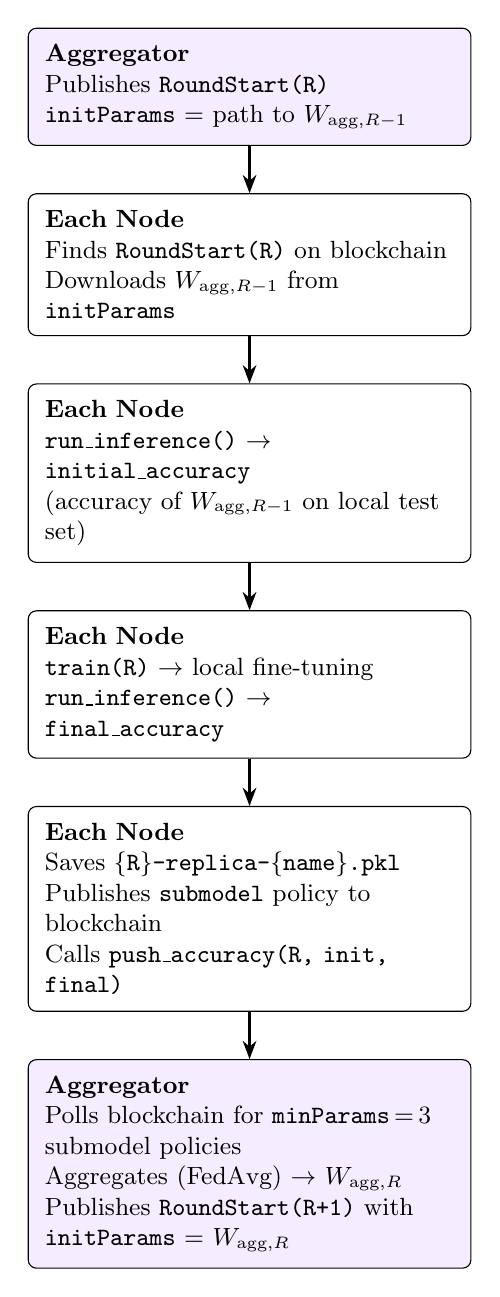
\begin{tikzpicture}[
    node distance=0.6cm and 1.5cm,
    box/.style={draw, rounded corners=3pt, fill=white,
                text width=5.2cm, align=left,
                font=\small, inner sep=6pt},
    aggbox/.style={draw, rounded corners=3pt, fill=aggpurple!40,
                   text width=5.2cm, align=left,
                   font=\small, inner sep=6pt},
    arr/.style={-Stealth, thick}
  ]

  \node[aggbox] (a1) {%
    \textbf{Aggregator}\\
    Publishes \texttt{RoundStart(R)}\\
    \texttt{initParams} $=$ path to \Wagg{R-1}
  };
  \node[box, below=of a1] (n1) {%
    \textbf{Each Node}\\
    Finds \texttt{RoundStart(R)} on blockchain\\
    Downloads \Wagg{R-1} from \texttt{initParams}
  };
  \node[box, below=of n1] (n2) {%
    \textbf{Each Node}\\
    \texttt{run\_inference()} $\rightarrow$ \texttt{initial\_accuracy}\\
    (accuracy of \Wagg{R-1} on local test set)
  };
  \node[box, below=of n2] (n3) {%
    \textbf{Each Node}\\
    \texttt{train(R)} $\rightarrow$ local fine-tuning\\
    \texttt{run\_inference()} $\rightarrow$ \texttt{final\_accuracy}
  };
  \node[box, below=of n3] (n4) {%
    \textbf{Each Node}\\
    Saves \texttt{\{R\}-replica-\{name\}.pkl}\\
    Publishes \texttt{submodel} policy to blockchain\\
    Calls \texttt{push\_accuracy(R, init, final)}
  };
  \node[aggbox, below=of n4] (a2) {%
    \textbf{Aggregator}\\
    Polls blockchain for \texttt{minParams}\,=\,3 submodel policies\\
    Aggregates (FedAvg) $\rightarrow$ \Wagg{R}\\
    Publishes \texttt{RoundStart(R+1)} with \texttt{initParams} $=$ \Wagg{R}
  };

  \draw[arr] (a1) -- (n1);
  \draw[arr] (n1) -- (n2);
  \draw[arr] (n2) -- (n3);
  \draw[arr] (n3) -- (n4);
  \draw[arr] (n4) -- (a2);

\end{tikzpicture}
\caption{Normal round lifecycle. Repeats for each round $R = 1 \ldots 10$.}
\end{figure}

\subsection{Round 1 special case}
In round\,1 the aggregator publishes \texttt{RoundStart(1)} with
\texttt{initParams = ``''} (empty string).  Each node detects
\texttt{round\_number == 1 and not aggregator\_model\_params\_db\_link}
and calls \texttt{get\_weights()} to obtain random initial weights
instead of downloading anything.  \texttt{initial\_accuracy} in round\,1
is therefore approximately $\frac{1}{10} \approx 10\%$ for 10-class MNIST
--- the model has not learned anything yet.

\newpage
% ═══════════════════════════════════════════════════════════════════════════════
\section{Round-by-Round Trace: Rounds 1--6 (Normal)}
\label{sec:normal}

\begin{tcolorbox}[infobox={Accuracy values}]
  The values below are \textbf{representative} for a 10-class MNIST run.
  Your exact numbers will differ, but the \emph{shape} of the curve
  (rapid rise early, then diminishing returns) should match.
  Node\,1 has a slightly harder data partition and converges more slowly.
\end{tcolorbox}

\begin{table}[H]
\centering
\small
\caption{Round-by-round summary, rounds 1--6}
\setlength{\tabcolsep}{5pt}
\begin{tabularx}{\textwidth}{c X c c c c c}
\toprule
\textbf{Round} & \textbf{Aggregator action} &
  \multicolumn{2}{c}{\textbf{Node 1}} &
  \multicolumn{2}{c}{\textbf{Nodes 2 \& 3 (avg)}} &
  \textbf{Produces} \\
\cmidrule(lr){3-4}\cmidrule(lr){5-6}
& & \texttt{global} & \texttt{train} & \texttt{global} & \texttt{train} & \\
\midrule
1 & Publishes \texttt{RoundStart(1)}, \texttt{initParams=""} &
  10.2\% & 52.4\% & 10.5\% & 55.1\% & \Wagg{1} \\
2 & \texttt{RoundStart(2)}, \texttt{initParams=}\Wagg{1} &
  57.3\% & 63.1\% & 58.6\% & 65.3\% & \Wagg{2} \\
3 & \texttt{RoundStart(3)}, \texttt{initParams=}\Wagg{2} &
  65.4\% & 70.2\% & 66.1\% & 71.8\% & \Wagg{3} \\
4 & \texttt{RoundStart(4)}, \texttt{initParams=}\Wagg{3} &
  70.1\% & 74.3\% & 71.4\% & 75.9\% & \Wagg{4} \\
5 & \texttt{RoundStart(5)}, \texttt{initParams=}\Wagg{4} &
  74.4\% & 77.6\% & 75.2\% & 78.7\% & \Wagg{5} \\
6 & \texttt{RoundStart(6)}, \texttt{initParams=}\Wagg{5} &
  \goodcell{77.2\%} & \goodcell{80.1\%} & \goodcell{78.3\%} & \goodcell{81.4\%} & \Wagg{6} \\
\bottomrule
\end{tabularx}
\end{table}

\noindent\textbf{What to observe in the logs (rounds 1--6):}

\begin{lstlisting}[style=log]
[mnist][Round 1] Listening for start round 1
[mnist][Round 1] Step 2 Complete: Model training done
[mnist][Round 1] Step 3 Complete: Model parameters published
[mnist][Round 1] Accuracy stored: initial=10.20%  final=52.40%  status=200
[mnist][Round 2] Listening for start round 2
...
[mnist][Round 6] Accuracy stored: initial=77.20%  final=80.10%  status=200
[mnist][Round 7] Listening for start round 7
\end{lstlisting}

\newpage
% ═══════════════════════════════════════════════════════════════════════════════
\section{Round 7: The Bad Round}
\label{sec:round7}

Round\,7 starts normally.  The aggregator publishes
\texttt{RoundStart(7)} with \texttt{initParams} pointing to \Wagg{6}.
All three nodes download \Wagg{6} and run inference.

\begin{table}[H]
\centering
\small
\caption{Round 7 per-node results}
\begin{tabular}{l c c c c}
\toprule
\textbf{Node} & \textbf{Starts from} & \textbf{global@node} &
  \textbf{after\_train} & \textbf{$\Delta$\_global} \\
\midrule
Node 1 & \Wagg{6} & \badcell{62.3\%} & \badcell{67.1\%} &
  \badcell{$-14.9\%$ ~\texttt{!}} \\
Node 2 & \Wagg{6} & 80.1\% & 83.2\% & $+1.8\%$ \\
Node 3 & \Wagg{6} & 79.8\% & 82.9\% & $+1.5\%$ \\
\bottomrule
\end{tabular}
\end{table}

\begin{tcolorbox}[rollbackbox={Interpreting the drop on Node 1}]
  Node\,1's \texttt{global@node} dropped from $77.2\%$ (round\,6) to
  $62.3\%$ (round\,7), a $\mathbf{-14.9\%}$ delta.
  The \texttt{!} marker in the accuracy report flags this.
  This means \Wagg{6} --- the aggregated model produced after round\,6 ---
  generalises poorly to Node\,1's local data distribution.
  Nodes\,2 and\,3 are unaffected; the issue is specific to Node\,1's partition.

  \medskip
  \textbf{What happened:} the aggregation in round\,6 likely shifted the
  global model toward Nodes\,2 and\,3's distribution at the expense of
  Node\,1.  This is the classic non-IID data imbalance effect in FedAvg.
\end{tcolorbox}

All three nodes still publish their round\,7 submodel policies.  The
aggregator collects all three (\texttt{minParams\,=\,3} satisfied),
runs FedAvg, and produces \Wagg{7}.  Round\,7 then completes normally
from the aggregator's perspective.

\medskip
\noindent After round\,7 completes on Node\,1:
\begin{itemize}[nosep]
  \item \texttt{round\_number["mnist"]} is now \textbf{8}.
  \item \texttt{listen\_for\_start\_round} is polling for
        \texttt{RoundStart(8)}.
  \item \texttt{\_rollback\_pending["mnist"]} is \texttt{False}.
\end{itemize}

\bigskip
\noindent\textbf{Accuracy report after round 7 (Node 1 only):}

\begin{lstlisting}[style=log]
============================================================
  index: mnist   node: node1
  global@node = accuracy of global model on this node's data (pre-train)
  delta_global = change vs previous round -- negative means rollback candidate
============================================================
  round  global@node  after_train  contributed   delta_global
  -----  -----------  -----------  -----------   ------------
      1        10.2%        52.4%       +42.2%            --
      2        57.3%        63.1%        +5.8%         +47.1
      3        65.4%        70.2%        +4.8%          +8.1
      4        70.1%        74.3%        +4.2%          +4.7
      5        74.4%        77.6%        +3.2%          +4.3
      6        77.2%        80.1%        +2.9%          +2.8
      7        62.3%        67.1%        +4.8%         -14.9  !
\end{lstlisting}

\noindent The \texttt{!} on round\,7 and the large negative delta are your
signal to check whether rollback is warranted.  In this test we decide it is.

\newpage
% ═══════════════════════════════════════════════════════════════════════════════
\section{Triggering the Manual Rollback}
\label{sec:trigger}

\subsection{Decision}

We want Node\,1 to start round\,8 from \Wagg{6} --- the last model where
Node\,1 had good accuracy --- instead of \Wagg{7}.

\begin{tcolorbox}[infobox={Why round 6?}]
  \texttt{POST /rollback \{"round": 6\}} instructs the node to load
  \Wagg{6}.  Internally \texttt{rollback\_to\_round} looks up
  \texttt{RoundStart(7)} on the blockchain (round $+ 1$) because that
  policy's \texttt{initParams} \emph{is} \Wagg{6}.  It fetches and loads
  those weights.
\end{tcolorbox}

\subsection{The curl command}

\begin{lstlisting}[style=bash]
# Target Node 1 only. Nodes 2 and 3 are not rolled back.
curl -X POST http://localhost:8080/rollback \
     -H "Content-Type: application/json" \
     -d '{"round": 6, "reason": "round 7 accuracy dropped -14.9% on node1"}'
\end{lstlisting}

\subsection{Expected response}

\begin{lstlisting}[style=json]
{
  "status": "success",
  "rolled_back_to_round": 6,
  "model_path": "/app/file_write/node1/mnist/7-agg_update.pkl",
  "message": "Model rolled back to round 6"
}
\end{lstlisting}

\subsection{What the code does internally (step by step)}

\begin{enumerate}
  \item \texttt{node\_server.py:414} --- \texttt{\_node\_ready.clear()}.
        The listener thread for Node\,1 blocks at
        \texttt{\_node\_ready.wait()} and will not start round\,8
        training until the rollback finishes.

  \item \texttt{rollback\_manager.py:105} ---
        \texttt{find\_roundstart\_policy("mnist", 7, el\_url)}
        queries the blockchain:\\
        \texttt{blockchain get mnist where round\_number = 7 and node\_type = aggregator}\\
        Returns the policy whose \texttt{initParams} $=$ \Wagg{6}.

  \item \texttt{rollback\_manager.py:129} ---
        \texttt{fetch\_and\_load\_weights} downloads \Wagg{6} using the same
        \texttt{copy\_file\_from\_container} / \texttt{read\_file} path as
        normal training.  Deserialises with \texttt{pickle.load},
        extracts \texttt{newUpdates}, calls \texttt{decode\_params},
        calls \texttt{data\_handlers["mnist"].update\_model(weights)}.

  \item \texttt{node.py:337--338} ---
        \texttt{\_rollback\_pending["mnist"] = True}\\
        \texttt{\_stale\_round["mnist"] = 6}

  \item \texttt{rollback\_manager.py:178} --- writes a row to the
        AnyLog \texttt{rollback\_events} table:\\
        \texttt{\{node\_name: "node1", trigger\_type: "manual",
        from\_round: 8, to\_round: 6, status: "success", ...\}}

  \item \texttt{node\_server.py:429} --- \texttt{\_node\_ready.set()}.
        Listener thread unblocks.
\end{enumerate}

\subsection{Node 1 state after rollback}

\begin{table}[H]
\centering
\small
\begin{tabular}{ll}
\toprule
\textbf{Field} & \textbf{Value} \\
\midrule
Active model weights & \Wagg{6} (rolled back) \\
\texttt{round\_number["mnist"]} & 8 (unchanged) \\
\texttt{\_rollback\_pending["mnist"]} & \texttt{True} \\
\texttt{\_stale\_round["mnist"]} & 6 \\
Listener polling for & \texttt{RoundStart(8)} \\
\bottomrule
\end{tabular}
\end{table}

\newpage
% ═══════════════════════════════════════════════════════════════════════════════
\section{Round 8: The Stale Round}
\label{sec:round8}

\begin{tcolorbox}[stalebox={Stale gradient warning}]
  Node\,1 is about to contribute a gradient computed from \Wagg{6},
  while Nodes\,2 and\,3 contribute gradients computed from \Wagg{7}.
  \Wagg{8} will be a \textbf{mixed-provenance aggregate}.
  This is an accepted trade-off at this stage of implementation.
  The staleness does not crash the system and training continues.
\end{tcolorbox}

\subsection{What happens when RoundStart(8) arrives on Node 1}

The aggregator publishes \texttt{RoundStart(8)} with
\texttt{initParams} $=$ \Wagg{7}.

Node\,1's listener thread, now unblocked, finds the policy at
\texttt{node\_server.py:205}.  Before calling
\texttt{train\_model\_params} it checks:

\begin{lstlisting}[style=bash]
skip_download = nodeInstance._rollback_pending.get("mnist", False)
# -> True
\end{lstlisting}

It logs the stale warning and clears the flag:

\begin{lstlisting}[style=log]
WARNING [mnist] Round 8: rollback active -- training from W_agg_6
        instead of W_agg_7. Stale gradient warning: aggregator will
        receive an update computed from an older global model.
\end{lstlisting}

\texttt{train\_model\_params} is called with \texttt{skip\_download=True}.
The \texttt{elif skip\_download} branch executes --- no download, no
\texttt{update\_model} call.  The model already holds \Wagg{6}.

\subsection{Round 8 execution per node}

\begin{table}[H]
\centering
\small
\caption{Round 8 per-node results}
\begin{tabular}{l c c c c c}
\toprule
\textbf{Node} & \textbf{Starts from} & \textbf{Downloads?} &
  \textbf{global@node} & \textbf{after\_train} & \textbf{$\Delta$\_global} \\
\midrule
\stalecell{Node 1} & \stalecell{\Wagg{6}} & \stalecell{No (stale)} &
  \stalecell{77.1\%} & \stalecell{80.0\%} & \stalecell{$+14.8\%$} \\
Node 2 & \Wagg{7} & Yes & 82.4\% & 84.6\% & $+2.3\%$ \\
Node 3 & \Wagg{7} & Yes & 82.1\% & 84.2\% & $+2.3\%$ \\
\bottomrule
\end{tabular}
\end{table}

\noindent\textbf{Node\,1's \texttt{global@node} for round\,8 is $\approx 77\%$} ---
the same level as round\,6 --- because the model it loaded \emph{is}
\Wagg{6}.  This is your confirmation the rollback worked: the accuracy
measurement reflects the rolled-back starting point.

\subsection{Aggregation of round 8}

All three nodes publish their round\,8 submodel policies.
The aggregator polls with \texttt{minParams\,=\,3} and collects all three.
No changes to the aggregator are needed:

\[
  W_{\text{agg},8}
  = \mathrm{FedAvg}\!\left(
      \underbrace{\theta_1^{(8)}}_{\text{from }\Wagg{6}},
      \underbrace{\theta_2^{(8)}}_{\text{from }\Wagg{7}},
      \underbrace{\theta_3^{(8)}}_{\text{from }\Wagg{7}}
    \right)
\]

The aggregator publishes \texttt{RoundStart(9)} with
\texttt{initParams} $=$ \Wagg{8}.

\subsection{After round 8: rollback state is cleared}

\texttt{\_rollback\_pending["mnist"]} was set to \texttt{False} before
the training call.  From round\,9 onward Node\,1 resumes normal behaviour
and downloads \texttt{initParams} as every other node does.

\newpage
% ═══════════════════════════════════════════════════════════════════════════════
\section{Rounds 9--10: Recovery}
\label{sec:recovery}

\begin{table}[H]
\centering
\small
\caption{Round-by-round summary, rounds 8--10}
\setlength{\tabcolsep}{5pt}
\begin{tabularx}{\textwidth}{c X c c c c c}
\toprule
\textbf{Round} & \textbf{Aggregator action} &
  \multicolumn{2}{c}{\textbf{Node 1}} &
  \multicolumn{2}{c}{\textbf{Nodes 2 \& 3 (avg)}} &
  \textbf{Produces} \\
\cmidrule(lr){3-4}\cmidrule(lr){5-6}
& & \texttt{global} & \texttt{train} & \texttt{global} & \texttt{train} & \\
\midrule
\stalecell{8} &
  \stalecell{\texttt{RoundStart(8)}, \texttt{initParams=}\Wagg{7}} &
  \stalecell{77.1\%} & \stalecell{80.0\%} &
  \stalecell{82.3\%} & \stalecell{84.4\%} &
  \stalecell{\Wagg{8} (mixed)} \\
9 & \texttt{RoundStart(9)}, \texttt{initParams=}\Wagg{8} &
  80.3\% & 82.6\% & 83.1\% & 85.0\% & \Wagg{9} \\
10 & \texttt{RoundStart(10)}, \texttt{initParams=}\Wagg{9} &
  82.1\% & 84.0\% & 84.7\% & 86.1\% & \Wagg{10} \\
\bottomrule
\end{tabularx}
\end{table}

\noindent The mixed aggregation in round\,8 produces \Wagg{8} that is
pulled slightly toward \Wagg{6} on Node\,1's component.
Rounds\,9 and\,10 normalise as all three nodes resume training from
the same global model.

\newpage
% ═══════════════════════════════════════════════════════════════════════════════
\section{Full Accuracy Report: Expected Output}
\label{sec:report}

Run this after all 10 rounds complete on any node to see the full table:

\begin{lstlisting}[style=bash]
curl http://localhost:8080/accuracy-report?index=mnist
\end{lstlisting}

\subsubsection*{Node 1}

\begin{lstlisting}[style=log]
============================================================
  index: mnist   node: node1
  global@node = accuracy of global model on this node's data (pre-train)
  delta_global = change vs previous round -- negative means rollback candidate
============================================================
  round  global@node  after_train  contributed   delta_global
  -----  -----------  -----------  -----------   ------------
      1        10.2%        52.4%       +42.2%             --
      2        57.3%        63.1%        +5.8%          +47.1
      3        65.4%        70.2%        +4.8%           +8.1
      4        70.1%        74.3%        +4.2%           +4.7
      5        74.4%        77.6%        +3.2%           +4.3
      6        77.2%        80.1%        +2.9%           +2.8
      7        62.3%        67.1%        +4.8%          -14.9  !   <-- trigger
      8        77.1%        80.0%        +2.9%          +14.8      <-- stale round
      9        80.3%        82.6%        +2.3%           +3.2
     10        82.1%        84.0%        +1.9%           +1.8
\end{lstlisting}

\subsubsection*{Nodes 2 \& 3 (unaffected by rollback)}

\begin{lstlisting}[style=log]
============================================================
  index: mnist   node: node2
============================================================
  round  global@node  after_train  contributed   delta_global
  -----  -----------  -----------  -----------   ------------
      1        10.5%        55.1%       +44.6%             --
      2        58.6%        65.3%        +6.7%          +48.1
      3        66.1%        71.8%        +5.7%           +7.5
      4        71.4%        75.9%        +4.5%           +5.3
      5        75.2%        78.7%        +3.5%           +3.8
      6        78.3%        81.4%        +3.1%           +3.1
      7        80.1%        83.2%        +3.1%           +1.8
      8        82.4%        84.6%        +2.2%           +2.3   <-- normal, no stale
      9        83.1%        85.0%        +1.9%           +0.7
     10        84.7%        86.1%        +1.4%           +1.6
\end{lstlisting}

\noindent Notice that Nodes\,2 and\,3 have no interruption at round\,8:
their \texttt{delta\_global} progresses normally.

\newpage
% ═══════════════════════════════════════════════════════════════════════════════
\section{Rollback History Endpoint}
\label{sec:history}

\begin{lstlisting}[style=bash]
curl http://localhost:8080/rollback/history?index=mnist
\end{lstlisting}

\begin{lstlisting}[style=json]
{
  "events": [
    {
      "node_name":    "node1",
      "index_name":  "mnist",
      "trigger_type": "manual",
      "from_round":   8,
      "to_round":     6,
      "reason":       "round 7 accuracy dropped -14.9% on node1",
      "status":       "success"
    }
  ]
}
\end{lstlisting}

\noindent \texttt{from\_round\,=\,8} because that was
\texttt{round\_number["mnist"]} at the time of the call --- the round
Node\,1 was \emph{about to} run when the rollback was triggered.
\texttt{to\_round\,=\,6} is the target.

\newpage
% ═══════════════════════════════════════════════════════════════════════════════
\section{Test Verification Checklist}
\label{sec:checklist}

Use this checklist when running the actual system.

\subsection{Before the rollback (rounds 1--7)}

\begin{itemize}
  \item[$\square$] All 3 nodes log \texttt{Listening for start round R}
        for each round --- confirms listener is alive.
  \item[$\square$] Aggregator logs \texttt{Step 4 Complete: model parameters
        aggregated} for rounds 1--7 --- confirms FedAvg ran every round.
  \item[$\square$] \texttt{GET /accuracy-report?index=mnist} on Node\,1 shows
        7 rows after round\,7 completes.
  \item[$\square$] Node\,1 round\,7 row has a large negative
        \texttt{delta\_global} with \texttt{!} marker.
  \item[$\square$] Nodes\,2 and\,3 round\,7 rows show no \texttt{!}.
\end{itemize}

\subsection{Triggering the rollback}

\begin{itemize}
  \item[$\square$] \texttt{POST /rollback \{"round": 6\}} on port\,8080
        (Node\,1) returns \texttt{"status": "success"}.
  \item[$\square$] Response contains \texttt{"rolled\_back\_to\_round": 6}.
  \item[$\square$] \texttt{GET /rollback/history?index=mnist} on Node\,1
        shows one event with
        \texttt{from\_round: 8, to\_round: 6, status: "success"}.
\end{itemize}

\subsection{Round 8 --- confirming the stale training path}

\begin{itemize}
  \item[$\square$] Node\,1 log contains the stale warning line:
  \begin{lstlisting}[style=log]
WARNING [mnist] Round 8: rollback active -- training from W_agg_6
        instead of W_agg_7. Stale gradient warning ...
  \end{lstlisting}
  \item[$\square$] Node\,1 log \textbf{does not} contain a download log line
        for round\,8 (no \texttt{copy\_file\_from\_container} /
        \texttt{read\_file} call should appear between the stale warning
        and the training-done message).
  \item[$\square$] Node\,1 round\,8 \texttt{global@node} is close to its
        round\,6 value ($\approx 77\%$), not its round\,7 value
        ($\approx 62\%$).  This confirms the model was not overwritten
        by \Wagg{7}.
  \item[$\square$] Nodes\,2 and\,3 round\,8 \texttt{global@node} continues
        to rise normally (no stale warning in their logs).
  \item[$\square$] Aggregator still produces \Wagg{8} after round\,8
        (\texttt{minParams\,=\,3} satisfied, all three submodel policies
        present on the blockchain).
\end{itemize}

\subsection{Rounds 9--10 --- confirming recovery}

\begin{itemize}
  \item[$\square$] Node\,1 log for round\,9 contains \textbf{no} stale
        warning --- confirms \texttt{\_rollback\_pending} was cleared.
  \item[$\square$] All three nodes' \texttt{delta\_global} values are
        positive in rounds\,9 and\,10.
  \item[$\square$] Node\,1 round\,9 \texttt{global@node} is above its
        round\,8 value --- confirms \Wagg{8} incorporated the
        mixed-provenance update and continued improving.
\end{itemize}

\newpage
% ═══════════════════════════════════════════════════════════════════════════════
\section{Quick Reference: All Curl Commands}
\label{sec:curl}

\begin{lstlisting}[style=bash]
# -- Accuracy report (any node) --
curl http://localhost:8080/accuracy-report?index=mnist
curl http://localhost:8081/accuracy-report?index=mnist
curl http://localhost:8082/accuracy-report?index=mnist

# -- Trigger manual rollback on Node 1 --
curl -X POST http://localhost:8080/rollback \
     -H "Content-Type: application/json" \
     -d '{"round": 6, "reason": "round 7 accuracy dropped"}'

# -- Check rollback history --
curl http://localhost:8080/rollback/history?index=mnist

# -- Check current rollback config --
curl http://localhost:8080/rollback/config

# -- Update rollback config at runtime (no restart needed) --
curl -X PUT http://localhost:8080/rollback/config \
     -H "Content-Type: application/json" \
     -d '{"patience_rounds": 3, "min_delta": 2.0}'
\end{lstlisting}

% ═══════════════════════════════════════════════════════════════════════════════
\section{Note on Decentralized FL}
\label{sec:decentralized}

The round lifecycle described in this document applies to the centralized
setup where one aggregator drives the \texttt{RoundStart} policies and all
nodes pull from it.

In a decentralized setup, nodes can act as both trainers and aggregators.
The rollback logic is \textbf{identical at the node level}:
\texttt{\_rollback\_pending}, \texttt{skip\_download},
\texttt{find\_roundstart\_policy}, and \texttt{fetch\_and\_load\_weights}
all function the same way regardless of who published the \texttt{RoundStart}
policy.  The difference is that in the decentralized case there is no single
aggregator to coordinate a global rollback --- each node rolls back
independently, and the stale gradient concern is magnified if multiple nodes
roll back simultaneously to different target rounds.
Coordinated multi-node rollback is deferred to a future implementation pass.

\bigskip
\begin{tcolorbox}[stalebox={Known limitation: stale gradient}]
  The current implementation intentionally introduces a stale gradient in
  round\,8 when a rollback is active.  Node\,1's contribution to \Wagg{8}
  is computed from \Wagg{6}, not \Wagg{7}.  The aggregator applies equal
  weight to all contributions and has no knowledge of the staleness.
  The effect on convergence is not yet measured.
  A follow-up pass will add a staleness tag to the submodel policy so the
  aggregator can apply a staleness discount (FedASMU pattern).
\end{tcolorbox}

\end{document}